\documentclass[a4paper,11pt]{report}
\usepackage{subcaption}
\usepackage{tikz}
\usetikzlibrary{cd}
%
\begin{document}
This is the first line
%\begin{center}
\begin{figure}[htb]
\centering
\begin{subfigure}[T]{0.4\textwidth}
\centering
\begin{tikzcd}
R \ar[r,leftarrow,"f"] \ar[rd,leftarrow, "f\circ x^{-1}"']  &U \ar[r,leftarrow,"\gamma"] \ar[d,"x"] &R \ar[dl, "        x       \circ\gamma"]\\
& R^d
\end{tikzcd}
\end{subfigure}
\centering  
\begin{subfigure}[T]{0.4\textwidth}
\centering
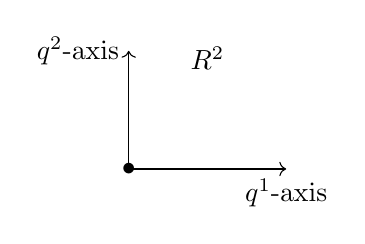
\begin{tikzpicture}
\node at (1,1.4){$R^2$};
\draw[->] (0,0)node{$\bullet$}--(2,0)node[below]{$q^1$-axis};
\draw[->] (0,0)--(0,1.5)node[left]{$q^2$-axis};
\end{tikzpicture}
\end{subfigure}
\caption{This is a test}
\end{figure}

%\end{center}
This is the last line.
\end{document}